\documentclass{ximera}

%\usepackage{todonotes}

\newcommand{\todo}{}

\usepackage{tkz-euclide}
\tikzset{>=stealth} %% cool arrow head
\tikzset{shorten <>/.style={ shorten >=#1, shorten <=#1 } } %% allows shorter vectors

\usepackage{tkz-tab}  %% sign charts
\usetikzlibrary{decorations.pathreplacing} 

\usetikzlibrary{backgrounds} %% for boxes around graphs
\usetikzlibrary{shapes,positioning}  %% Clouds and stars
\usetikzlibrary{matrix} %% for matrix
\usepgfplotslibrary{polar} %% for polar plots
\usetkzobj{all}
\usepackage[makeroom]{cancel} %% for strike outs
%\usepackage{mathtools} %% for pretty underbrace % Breaks Ximera
\usepackage{multicol}

\usepackage{polynom}



\usepackage[many]{tcolorbox}  %% for titled boxes
\newtcolorbox{xbox}[1]{%
    tikznode boxed title,
    enhanced,
    arc=0mm,
    interior style={white},
    attach boxed title to top center= {yshift=-\tcboxedtitleheight/2},
    fonttitle=\bfseries,
    colbacktitle=white,coltitle=black,
    boxed title style={size=normal,colframe=white,boxrule=0pt},
    title={#1}}


\usepackage{array}
\setlength{\extrarowheight}{+.1cm}   
\newdimen\digitwidth
\settowidth\digitwidth{9}
\def\divrule#1#2{
\noalign{\moveright#1\digitwidth
\vbox{\hrule width#2\digitwidth}}}





\newcommand{\RR}{\mathbb R}
\newcommand{\R}{\mathbb R}
\newcommand{\N}{\mathbb N}
\newcommand{\Z}{\mathbb Z}

%\renewcommand{\d}{\,d\!}
\renewcommand{\d}{\mathop{}\!d}
\newcommand{\dd}[2][]{\frac{\d #1}{\d #2}}
\newcommand{\pp}[2][]{\frac{\partial #1}{\partial #2}}
\renewcommand{\l}{\ell}
\newcommand{\ddx}{\frac{d}{\d x}}
\newcommand{\ddt}{\frac{d}{\d t}}

\newcommand{\zeroOverZero}{\ensuremath{\boldsymbol{\tfrac{0}{0}}}}
\newcommand{\inftyOverInfty}{\ensuremath{\boldsymbol{\tfrac{\infty}{\infty}}}}
\newcommand{\zeroOverInfty}{\ensuremath{\boldsymbol{\tfrac{0}{\infty}}}}
\newcommand{\zeroTimesInfty}{\ensuremath{\small\boldsymbol{0\cdot \infty}}}
\newcommand{\inftyMinusInfty}{\ensuremath{\small\boldsymbol{\infty - \infty}}}
\newcommand{\oneToInfty}{\ensuremath{\boldsymbol{1^\infty}}}
\newcommand{\zeroToZero}{\ensuremath{\boldsymbol{0^0}}}
\newcommand{\inftyToZero}{\ensuremath{\boldsymbol{\infty^0}}}



\newcommand{\numOverZero}{\ensuremath{\boldsymbol{\tfrac{\#}{0}}}}
\newcommand{\dfn}{\textbf}
%\newcommand{\unit}{\,\mathrm}
\newcommand{\unit}{\mathop{}\!\mathrm}
\newcommand{\eval}[1]{\bigg[ #1 \bigg]}
\newcommand{\seq}[1]{\left( #1 \right)}
\renewcommand{\epsilon}{\varepsilon}
\renewcommand{\iff}{\Leftrightarrow}

\DeclareMathOperator{\arccot}{arccot}
\DeclareMathOperator{\arcsec}{arcsec}
\DeclareMathOperator{\arccsc}{arccsc}
\DeclareMathOperator{\si}{Si}
\DeclareMathOperator{\proj}{proj}
\DeclareMathOperator{\scal}{scal}


\newcommand{\tightoverset}[2]{% for arrow vec
  \mathop{#2}\limits^{\vbox to -.5ex{\kern-0.75ex\hbox{$#1$}\vss}}}
\newcommand{\arrowvec}[1]{\tightoverset{\scriptstyle\rightharpoonup}{#1}}
\renewcommand{\vec}{\mathbf}
\newcommand{\veci}{\vec{i}}
\newcommand{\vecj}{\vec{j}}
\newcommand{\veck}{\vec{k}}
\newcommand{\vecl}{\boldsymbol{\l}}

\newcommand{\dotp}{\bullet}
\newcommand{\cross}{\boldsymbol\times}
\newcommand{\grad}{\boldsymbol\nabla}
\newcommand{\divergence}{\grad\dotp}
\newcommand{\curl}{\grad\cross}
%\DeclareMathOperator{\divergence}{divergence}
%\DeclareMathOperator{\curl}[1]{\grad\cross #1}


\colorlet{textColor}{black} 
\colorlet{background}{white}
\colorlet{penColor}{blue!50!black} % Color of a curve in a plot
\colorlet{penColor2}{red!50!black}% Color of a curve in a plot
\colorlet{penColor3}{red!50!blue} % Color of a curve in a plot
\colorlet{penColor4}{green!50!black} % Color of a curve in a plot
\colorlet{penColor5}{orange!80!black} % Color of a curve in a plot
\colorlet{fill1}{penColor!20} % Color of fill in a plot
\colorlet{fill2}{penColor2!20} % Color of fill in a plot
\colorlet{fillp}{fill1} % Color of positive area
\colorlet{filln}{penColor2!20} % Color of negative area
\colorlet{fill3}{penColor3!20} % Fill
\colorlet{fill4}{penColor4!20} % Fill
\colorlet{fill5}{penColor5!20} % Fill
\colorlet{gridColor}{gray!50} % Color of grid in a plot

\newcommand{\surfaceColor}{violet}
\newcommand{\surfaceColorTwo}{redyellow}
\newcommand{\sliceColor}{greenyellow}




\pgfmathdeclarefunction{gauss}{2}{% gives gaussian
  \pgfmathparse{1/(#2*sqrt(2*pi))*exp(-((x-#1)^2)/(2*#2^2))}%
}


%%%%%%%%%%%%%
%% Vectors
%%%%%%%%%%%%%

%% Simple horiz vectors
\renewcommand{\vector}[1]{\left\langle #1\right\rangle}


%% %% Complex Horiz Vectors with angle brackets
%% \makeatletter
%% \renewcommand{\vector}[2][ , ]{\left\langle%
%%   \def\nextitem{\def\nextitem{#1}}%
%%   \@for \el:=#2\do{\nextitem\el}\right\rangle%
%% }
%% \makeatother

%% %% Vertical Vectors
%% \def\vector#1{\begin{bmatrix}\vecListA#1,,\end{bmatrix}}
%% \def\vecListA#1,{\if,#1,\else #1\cr \expandafter \vecListA \fi}

%%%%%%%%%%%%%
%% End of vectors
%%%%%%%%%%%%%

%\newcommand{\fullwidth}{}
%\newcommand{\normalwidth}{}



%% makes a snazzy t-chart for evaluating functions
%\newenvironment{tchart}{\rowcolors{2}{}{background!90!textColor}\array}{\endarray}

%%This is to help with formatting on future title pages.
\newenvironment{sectionOutcomes}{}{} 



%% Flowchart stuff
%\tikzstyle{startstop} = [rectangle, rounded corners, minimum width=3cm, minimum height=1cm,text centered, draw=black]
%\tikzstyle{question} = [rectangle, minimum width=3cm, minimum height=1cm, text centered, draw=black]
%\tikzstyle{decision} = [trapezium, trapezium left angle=70, trapezium right angle=110, minimum width=3cm, minimum height=1cm, text centered, draw=black]
%\tikzstyle{question} = [rectangle, rounded corners, minimum width=3cm, minimum height=1cm,text centered, draw=black]
%\tikzstyle{process} = [rectangle, minimum width=3cm, minimum height=1cm, text centered, draw=black]
%\tikzstyle{decision} = [trapezium, trapezium left angle=70, trapezium right angle=110, minimum width=3cm, minimum height=1cm, text centered, draw=black]



\title[Dig-In:]{Explanation of the product and chain rules}

\begin{document}
\begin{abstract}
  We give explanation for the product rule and chain rule.
\end{abstract}
\maketitle


Now that we know about differentials, let's use them to give some
intuition as to why the product and chain rules are true.


\section{Explanation of the product rule}

Linear approximations can help us explain why the product rule works.

\begin{theorem}[The product rule]\index{product rule}
If $f$ and $g$ are differentiable, then
\[
\ddx f(x)g(x) = f(x)g'(x)+f'(x)g(x).
\]
\begin{explanation}
  To start, we need some way to understand the function
  \[
  A(x) = f(x) \cdot g(x).
  \]
  One interpretation of multiplication is it is the area of a $f(x)
  \times g(x)$ rectangle:
  \begin{image}
    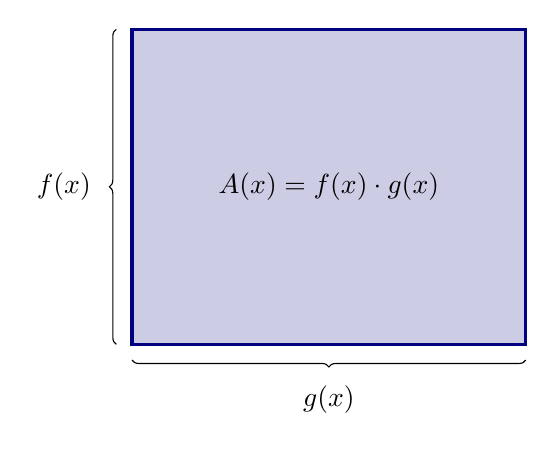
\begin{tikzpicture}
      \draw [penColor,very thick,fill=fill1] (0,0) rectangle (5,4);
      \node at (2.5,2) {$A(x) = f(x) \cdot g(x)$};
      \draw [decoration={brace,mirror,raise=.2cm},decorate,thin] (0,0)--(5,0);
      \draw [decoration={brace,raise=.2cm},decorate,thin] (0,0)--(0,4);
      \node [below] at (2.5,-.4) {$g(x)$};
      \node [left] at (-.4,2) {$f(x)$};
    \end{tikzpicture}
  \end{image}
  To understand the derivative of the product, we must understand how
  the area, $A$, changes as $x$ changes. If we change the inputs of
  $f$ and $g$ by $\d x$, then the size of the rectangle changes:
  \begin{image}
    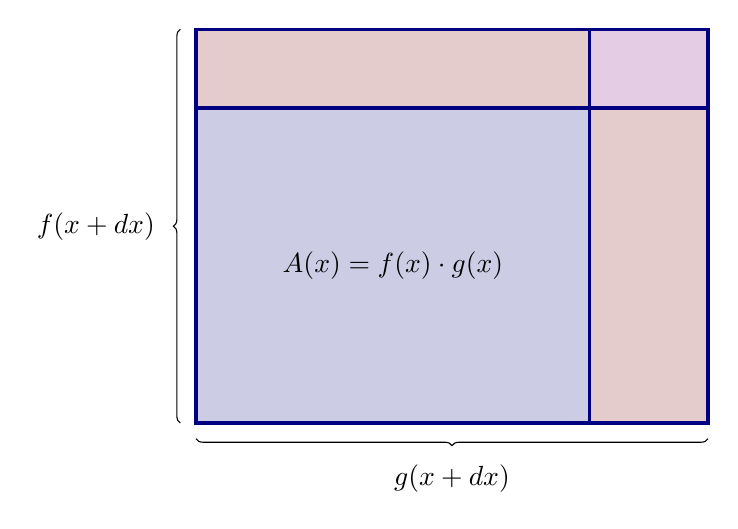
\begin{tikzpicture}
      \draw [penColor,very thick,fill=fill1] (0,0) rectangle (5,4);
      \draw [penColor,very thick,fill=fill2] (5,0) rectangle (6.5,5);
      \draw [penColor,very thick,fill=fill2] (0,4) rectangle (6.5,5);
      \draw [penColor,very thick,fill=fill3] (5,4) rectangle (6.5,5);
      \node at (2.5,2) {$A(x) = f(x) \cdot g(x)$};
      \draw [decoration={brace,mirror,raise=.2cm},decorate,thin] (0,0)--(6.5,0);
      \draw [decoration={brace,raise=.2cm},decorate,thin] (0,0)--(0,5);
      \node [below] at (3.25,-.4) {$g(x+\d x)$};
      \node [left] at (-.4,2.5) {$f(x+ \d x)$};
    \end{tikzpicture}
  \end{image}
  However, we know from our previous work that
  \begin{align*}
    f(x+\d x) &\approx f(x) + \d f,\\
    g(x+\d x) &\approx g(x) + \d g,\\
  \end{align*}
  so now our picture becomes:
  \begin{image}
    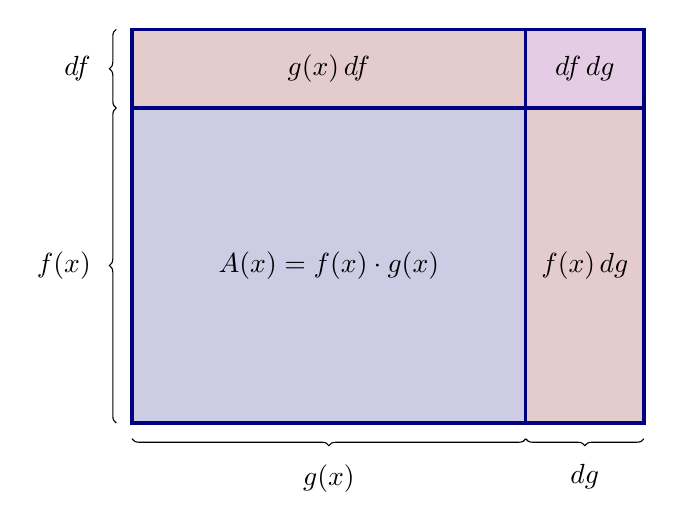
\begin{tikzpicture}
      \draw [penColor,very thick,fill=fill1] (0,0) rectangle (5,4);
      \draw [penColor,very thick,fill=fill2] (5,0) rectangle (6.5,5);
      \draw [penColor,very thick,fill=fill2] (0,4) rectangle (6.5,5);
      \draw [penColor,very thick,fill=fill3] (5,4) rectangle (6.5,5);

      \node at (2.5,2) {$A(x) = f(x) \cdot g(x)$};
      \node at (2.5,4.5) {$g(x)\d f$};
      \node at (5.75,2) {$f(x) \d g$};
      \node at (5.75,4.5) {$\d f\d g$};

      
      \draw [decoration={brace,mirror,raise=.2cm},decorate,thin] (0,0)--(5,0);
      \draw [decoration={brace,raise=.2cm},decorate,thin] (0,0)--(0,4);
      \node [below] at (2.5,-.4) {$g(x)$};
      \node [left] at (-.4,2) {$f(x)$};
      \draw [decoration={brace,mirror,raise=.2cm},decorate,thin] (5,0)--(6.5,0);
      \draw [decoration={brace,raise=.2cm},decorate,thin] (0,4)--(0,5);
      \node [below] at (5.75,-.4) {$\d g$};
      \node [left] at (-.4,4.5) {$\d f$};
    \end{tikzpicture}
  \end{image}
  Note, if we think of $A(x) = f(x)\cdot g(x)$, then we can also label
  our picture as follows:
  \begin{image}
    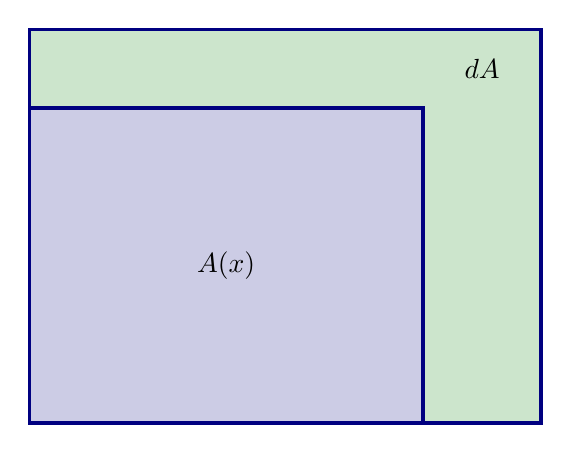
\begin{tikzpicture}
      \draw [penColor,very thick,fill=fill4] (0,0) rectangle (6.5,5);
      \draw [penColor,very thick,fill=fill1] (0,0) rectangle (5,4);
     
      \node at (2.5,2) {$A(x)$};
      \node at (5.75,4.5) {$\d A$};
    \end{tikzpicture}
  \end{image}
  Finally, from the pictures above and recalling that
  \begin{align*}
    \d f &= f'(x) \d x\\
    \d g &= g'(x) \d x,
  \end{align*}
  we see that
  \begin{align*}
    \d A &= f(x) \d g + g(x) \d f + \d f \d g\\
    &=f(x) g'(x) \d x + g(x) f'(x) \d x + f'(x) g'(x) \left(\d x\right)^2.
  \end{align*}
  Dividing both sides by $\d x$ we see
  \[
  \dd[A]{x} = f(x) g'(x) + g(x) f'(x) + f'(x) g'(x) \d x
  \]
  and letting $\d x$ go to zero we see
  \[
  A'(x) = f(x) g'(x) + g(x) f'(x).
  \]
\end{explanation}
\end{theorem}    



\section{Explanation of the chain rule}

Now we'll use linear approximations to help explain why the chain rule
is true.

\begin{theorem}[Chain Rule]\index{chain rule}
If $f$ and $g$ are differentiable, then
\[
\ddx f(g(x)) = f'(g(x))g'(x).
\]
\begin{explanation}
  We'll try to understand this geometrically. In what follows, the
  functions $f$ and $g$ look like lines; however, the young
  mathematician should realize that we are \textbf{not} looking at true
  lines, instead we are looking at $f$ and $g$ sufficiently
  ``zoomed-in'' so that they appear to be lines.  First consider a
  graph of $g$ with respect to $x$:
  \begin{image}
    \begin{tikzpicture}
      \begin{axis}[
          domain=-.1:2,
          ymin=-.1,
          ymax=4,
          xtick={.75}, 
          xticklabels={$x$},
          ytick={1.5},
          yticklabels={$g(x)$},
          axis lines =middle, %xlabel=, ylabel=$y$,
          every axis y label/.style={at=(current axis.above origin),anchor=south},
          every axis x label/.style={at=(current axis.right of origin),anchor=west},
        ]
	\addplot [very thick, penColor2] {2*x};
        \addplot [textColor!50!background] plot coordinates {(.75,0) (.75,1.5)};
        \addplot [textColor!50!background] plot coordinates {(.75,1.5) (0,1.5)};
        
        \addplot [dashed,->] plot coordinates {(.75,2*.75) (1.25,2*.75)};
        \addplot [dashed,->] plot coordinates {(1.25,2*.75) (1.25,2*1.25)};

        \node at (axis cs:1,2*.75) [anchor=north] {$\d x$};
        \node at (axis cs:1.25,2) [anchor=west] {$\d g$};

        \addplot[color=penColor2,fill=penColor2,only marks,mark=*] coordinates{(.75,1.5)};  %% closed hole         
      \end{axis}
    \end{tikzpicture}
  \end{image}
  Now consider a graph of $f$ with respect to $g$:
  \begin{image}
    \begin{tikzpicture}
      \begin{axis}[
          domain=-.1:2,
          ymin=-.1,
          ymax=4,
          xtick={1}, 
          xticklabels={$g$},
          ytick={3},
          yticklabels={$f(g)$},
          axis lines =middle, %xlabel=, ylabel=$y$,
          every axis y label/.style={at=(current axis.above origin),anchor=south},
          every axis x label/.style={at=(current axis.right of origin),anchor=west},
        ]
	\addplot [very thick, penColor] {2+x};
        \addplot [textColor!50!background] plot coordinates {(1,0) (1,3)};
        \addplot [textColor!50!background] plot coordinates {(1,3) (0,3)};
        
        \addplot [dashed,->] plot coordinates {(1,3) (1.5,3)};
        \addplot [dashed,->] plot coordinates {(1.5,3) (1.5,3.5)};

        \node at (axis cs:1.25,3) [anchor=north] {$\d g$};
        \node at (axis cs:1.5,3.25) [anchor=west] {$\d f$};

        \addplot[color=penColor,fill=penColor,only marks,mark=*] coordinates{(1,3)};  %% closed hole         
      \end{axis}
    \end{tikzpicture}
  \end{image}
  If we combine these graphs, by laying the graph of $g$ on its side,
  we obtain:
  \begin{image}
    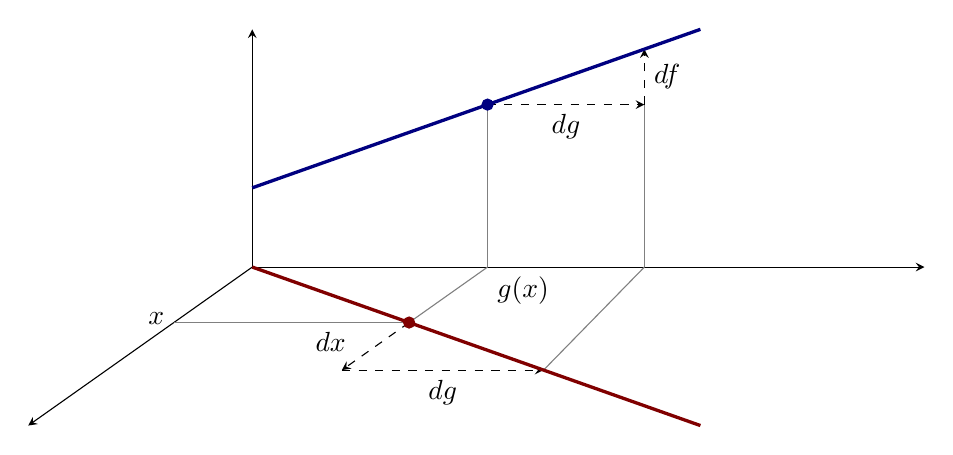
\begin{tikzpicture}
      \begin{axis}[
          axis lines=none,
          clip=false,
          width=6in,
          height=3in,
        ]          
        \addplot [->,textColor] plot coordinates {(0,0) (-2,-4)}; %% x axis
        \addplot [->,textColor] plot coordinates {(0,0) (0,6)}; %% y axis
        \addplot [->,textColor] plot coordinates {(0,0) (6,0)}; %% g axis
        
        \addplot [textColor!50!background] plot coordinates {(-.7,-1.4) (1.4,-1.4)};
        \addplot [textColor!50!background] plot coordinates {(1.4,-1.4) (2.1,0)};
        \addplot [textColor!50!background] plot coordinates {(2.1,0) (2.1,4.1)};
        
        \addplot [textColor!50!background] plot coordinates {(2.6,-2.6) (3.5,0)};
        \addplot [textColor!50!background] plot coordinates {(3.5,0) (3.5,4.1)};
        
        \addplot [dashed,->] plot coordinates {(1.4,-1.4) (.8,-2.6)};
        \addplot [dashed,->] plot coordinates {(2.1,4.1) (3.5,4.1)};
        
        \addplot [dashed,->] plot coordinates {(.8,-2.6) (2.6,-2.6)};
        \addplot [dashed,->] plot coordinates {(3.5,4.1) (3.5,5.5)};

        \addplot [very thick,penColor,domain=(0:4)] {2+x};
        \addplot [very thick,penColor2,domain=(0:4)] {-x};
        
        \node at (axis cs:3.5,4.8) [anchor=west] {$\d f$};
        \node at (axis cs:1.7,-2.6) [anchor=north] {$\d g$};
        \node at (axis cs:2.8,4.1) [anchor=north] {$\d g$};
        \node at (axis cs:2.1,0) [anchor=north west] {$g(x)$};
        
        \addplot[color=penColor2,fill=penColor2,only marks,mark=*] coordinates{(1.4,-1.4)};  %% closed hole          
        \addplot[color=penColor,fill=penColor,only marks,mark=*] coordinates{(2.1,4.1)};  %% closed hole
        %\addplot[color=penColor3,fill=penColor3,only marks,mark=*] coordinates{(2.1,0)};  %% closed hole          
        
        %\node at (axis cs:1,-2.1) [anchor=south,yslant=0,xslant=0,rotate=53] {$\overbrace{\hspace{.36in}}^{h}$};
        \node at (axis cs:.7,-1.9) {$\d x$};
        
        %\node at (axis cs:7,0) [anchor=east] {$g(x)$};
        %\node at (axis cs:0,6.7) [anchor=north] {$y$};
        %\node at (axis cs:-2.15,-4) [anchor=north] {$x$};
        \node at (axis cs:-.7,-1.3) [anchor=east] {$x$};
      \end{axis}
    \end{tikzpicture}
  \end{image}
  Ah! From this we see that
  \begin{align*}
    \d f &= f'(g) \d g\\
    &= f'(g(x)) g'(x) \d x,
  \end{align*}
  so
  \[
  \dd[f]{x} = f'(g(x))g'(x).
  \]
\end{explanation}
\end{theorem}


These ``explanations'' are not meant to be the end of the story for
the product rule and chain rule, rather they are hopefully the
beginning. As you learn more mathematics, these explanations will be
refined and made precise.



%% %% HERE I TRIED TO GIVE A NICE CONCEPTUAL EXPLANATION OF THE CHAIN RULE AND FAILED.
%%
%% We can think about this explanation in a sightly different way.
%% Consider this
%% \begin{align*}
%% g'(x) &= \text{how $g$ changes as $x$ changes,}\\
%% f'(g) &= \text{how $f$ changes as $g$ changes,}
%% \end{align*}
%% and to be more explicit
%% \begin{align*}
%% g'(x) &= \frac{\text{(how $g$ changes)}}{\text{(how $x$ changes)}},\\
%% f'(g) &= \frac{\text{(how $f$ changes)}}{\text{(how $g$ changes)}}.
%% \end{align*}
%% hence if we want to know
%% \begin{quote}
%%   How $f$ changes as $g$ changes as $x$ changes.
%% \end{quote}
%% Then we 
%% \[
%% \ddx f(g(x)) = \frac{\text{(how $f$ changes)}}{\text{(how $g$ changes)}}\cdot\frac{\text{(how $g$ changes)}}{\text{(how $x$ changes)}}
%% \]
%% $= f'(g(x)) g'(x).$



%% Let's continue along these lines and put a real-context to it. If 
%% \[
%% g(m) = \text{the amount of gas one can buy with $m$ dollars,}
%% \]
%% and
%% \[
%% f(g) = \text{how far one can drive with $g$ gallons of gas,}
%% \]
%% then $f(g(m))$ represents how far one can drive with $m$ dollars. If we
%% ask ourselves how is $f\circ g$ changing as $m$ changes, we can reason
%% as follows:

%% The distance we can travel with $g$ gallons of gas changes at a rate
%% relative to the amount of gas we currently have. This is represented by
%% \[
%% f'(g(m)).
%% \]
%% However, as we change the amount $m$ of money used, 



\end{document}
